\chapter{Niveau 2 : La Tombe Supérieure}\label{n2}
\section{Structure}
Cette section est toujours linéaire, mais avec plus de pièces annexes et quelques dangers environnementaux.
Le chemin "vers l'avant" est toujours clair, mais les salles annexes sont tentantes.
C'est ici que les leçons du Niveau 1 sont évaluées et mises en pratique.

Cet étage devrait prendre 2 ou 3 sessions à explorer, et peut requérir un trajet de retour à la civilisation pour faire le plein.


\section{Zones Thématiques}
\subsection{La Vraie Tombe}
\begin{itemize}
  \item Représente le pouvoir et les menaces implicites.
  \item Des statues veillent.
  \item Des choses tressaillent dans leurs cercueils scellés.
  \item Des lézards géants vous traquent dans l'obscurité, des sorciers immortels proposent des pactes indicibles et d'invincibles mucus morts-vivants serpentent à votre poursuite.
\end{itemize}

Décrivez cette zone avec des mots comme "énorme", "menaçant" et "froid".

C'est l'\oe uvre d'une civilisation bien plus ancienne, sage et cruelle que celle des PJ.
Plus ils s'enfoncent profondément, plus la tension devrait les rendre nerveux.
\vfill
\subsection{Le Gouffre}
Incarne l'inconnu, et ses promesses.
Il pourrait y avoir n'importe quoi en bas
\begin{itemize}
  \item Le centre de la Terre;
  \item Des hommes-serpents vivant toujours paisiblement dans les profondeurs
  \item etc.
\end{itemize}
C'est la toile vierge du module, sur laquelle le MJ peut venir ajouter ce que bon lui semble.

Décrivez le gouffre avec des mots comme \emph{"sans fond"}, \emph{"vertigineux, comme si le monde entier s'écroulait"} et \emph{"résonnant de lointains mais persistants échos, si vous êtes patients"}.

Les PJ ne devraient pas vouloir passer plus de temps que nécessaire au bord de l'abîme.


\ifmulticolEnd
\begin{center}
  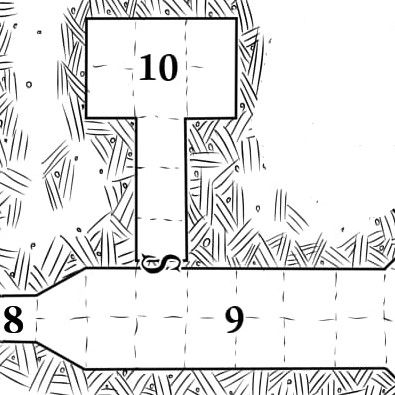
\includegraphics[width=0.6\linewidth]{pics/map_8-10.jpg}
\end{center}
\ifmulticolStart

\subsection{8 : Passage Secret}\label{n2:s8}
\begin{itemize}
  \item 9m de long sur 3m, 1.5m de haut
  \item Directement sous \textbf{\nameref{n1:s7}}
  \item \'Etroite alcôve s'élargissant sur \textbf{\nameref{n2:s9}}
  \item Sent le \textbf{moisi},et la \textbf{pierre humide}
  \item \textbf{Roche taillée finement}, mais gâchée par des fissures causées par l'eau.
  \item Flaques au sol.
\end{itemize}

\subsection{9 : Hall aux Statues}\label{n2:s9}
Un long et large couloir.
\begin{itemize}
  \item 21m de long sur 6m, 5m de haut
  \item Sent le \textbf{moisi},et la \textbf{pierre humide}
  \item Mince filet d'eau coule vers l'est
  \item Six énormes \textbf{statues d'hommes-serpents} en armes et armures
  \begin{itemize}
    \item Regard dédaigneux
    \item 1\iere{} à gauche : légèrement désalignée
    \item déplacée, révèle \textbf{\nameref{n2:s10}}
  \end{itemize}
\end{itemize}

\vfill
\subsection{10 : Salle de Garde Secrète}\label{n2:s10}
Cette pièce fut autrefois une salle de garde secrète pour les assassins du temple.

\begin{itemize}
  \item Salle de 9m sur 6m, 3m de haut
  \item Sent le \textbf{bois pourrissant},et le \textbf{tissu putréfié}
  \item Vide et sombre.
  \item Les meubles ont pourri jusqu'à se désagréger.
  \item Deux guisarmes sont toujours utilisables
  \item Une icône religieuse en argent valant 50 PO.
\end{itemize}

\vfill\pagebreak
\subsection{11 : Atrium des Tombes}\label{n2:s11}
\begin{itemize}
    \item Pièce \textbf{octogonale}, avec une ouverture au sud ouest, des portes sur les autres côtés
    \item 18m sur 18m, 5m de haut
    \item Sent le \textbf{réglisse} et la \textbf{décomposition}
    \item Bordée de statues scrutatrices d'hommes-serpents
    \item Porte Sud-Est en bois
    \item Porte Est en pierre finement ouvragée: gravures de serpents pleuvant des cieux.
    \item Autres scellées par d'épaisses portes de pierre
    \begin{itemize}
        \item tombe aisément en faisant levier
    \end{itemize}
    \item Au centre \textbf{bassin empli d'eau} de 2m de diamètre
    \begin{itemize}
        \item Eau \textbf{sombre} et \textbf{huileuse} qui sent la \textbf{réglisse}
        \item Profond de 3m
        \item 2 \textbf{\nameref{monster:s11}}, bondissent et attaquent quiconque s'approche
    \end{itemize}
\end{itemize}



Toucher l'eau ne déclenche pas de pourriture momifiante, mais la boire ou la mettre en contact avec une blessure ouverte, si.

Le bassin contient :
\begin{enumerate}
    \item Une \textbf{tête de momie} en furie qui a sombré depuis longtemps dans la folie ;
    \item Une lourde \textbf{chaîne d'or} valant 350 PO ;
    \item Un \textbf{anneau magique} en argent ;
    \item Un \textbf{outil magique} au choix du MJ ou aléatoire, ou 2d10x10 PO de joaillerie.
\end{enumerate}

\begin{center}
  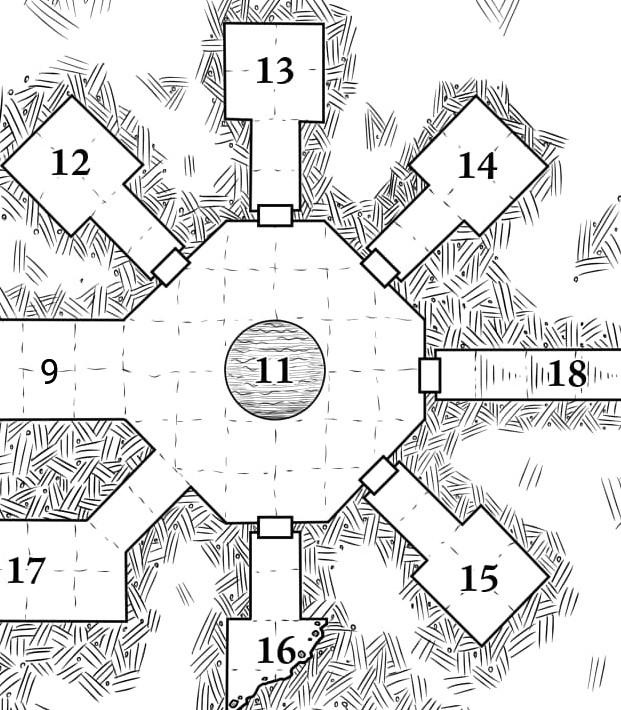
\includegraphics[width=0.9\linewidth]{pics/map_11-18.jpg}
\end{center}

\vfill

\begin{highlight}[Anneau d'argent : bague de vision]
Enfilée au doigt, l'un des yeux du porteur jaillit de son orbite, et devient dur comme du verre.
L'\oe il voit toujours normalement.
\end{highlight}


\subsection{12 : Tombe de Xisor le Vert}\label{n2:s12}
\subsubsection{Passage}
\begin{itemize}
    \item Odeur d'\textbf{ozone}
    \item \textbf{Dalle piégée} dans le passage
    \item Active un sort d'\textbf{éclair}, vers l'entrée du couloir (4d6 dégâts, 2d6 si sauvegarde Sorts)
    \item Activé une seule fois
    \item Tiré depuis une \textbf{plaque d'électrum} dans le mur (100PO)
\end{itemize}
\subsubsection{Tombe}
\begin{itemize}
  \item Salle de 6m sur 6m, 3m de haut
  \item Sent les \textbf{épices d'embaumement}
  \item 1 \textbf{cercueil de pierre}
\end{itemize}
Un parchemin de sort (venin oculaire, ou autre sort basé sur le venin) se trouve dans le
cercueil de Xisor.

%\vfill\columnbreak
\subsection{13 : Tombe de Sparamantur}\label{n2:s13}
\begin{itemize}
  \item Salle de 6m sur 6m, 3m de haut
  \item Porte de pierre brisée
  \item Passage partiellement \textbf{effondré}
  \item Si excavation : \textbf{sons d'agitation} de l'autre côté
  \item \textbf{\nameref{monster:s13}} attaque à vue
  \begin{itemize}
    \item Squelette homme-serpent
  \end{itemize}
  \item Ses ornements funéraires valent 100 PO
\end{itemize}

\subsection{14 : Tombe de Franbinzar}\label{n2:s14}
\begin{itemize}
    \item Salle de 6m sur 6m, 3m de haut
    \item Sent le \textbf{goudron} et la \textbf{décomposition}.
    \item Tombe décorée de \textbf{peintures} et \textbf{gravures obscènes}
    \item \textbf{Cercueil de pierre :} restes de \textbf{\nameref{monster:s14}} (Pudding Noir)
    \begin{itemize}
      \item \textbf{Ouverture :} attaque
      \item \textbf{Trésor :} copies d'argile, mais 200 PO d'anneaux sont noyés dans sa masse
    \end{itemize}
\end{itemize}

Si Franbinzar a été libéré, il est ajouté à la Table des \textbf{\nameref{monster:n3:errants}} à la place d'un des présages.

\vfill\columnbreak

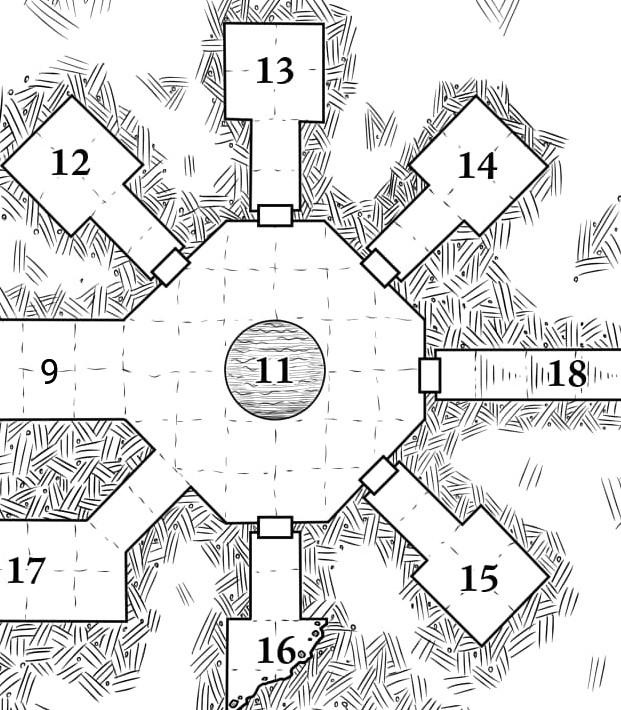
\includegraphics[width=\linewidth]{pics/map_11-18.jpg}

\subsection{15 : Sacristie}\label{n2:s15}
Cette pièce était utilisée par les prêtres de la tombe supérieure.
\begin{itemize}
  \item Salle de 6m sur 6m, 3m de haut
  \item Sent le \textbf{bois pourrissant} et la \textbf{poussière}.
\end{itemize}
Elle contient :
\begin{itemize}
    \item Trois lits,
    \item Des étagères vermoulues,
    \item Une icône religieuse de dieu-serpent en argent et émeraude (200 PO)
    \item Parchemins en langue inconnue (témoignent de la folie des momies emprisonnées).
          Éparpillés au sol.
          \begin{itemize}
            \item l'un contient le nom de la \textbf{\nameref{monster:n3:succube}} piégée en \textbf{\nameref{n3:s32}}
          \end{itemize}
\end{itemize}

\subsection{16 : Tombe Inachevée}\label{n2:s16}
\begin{itemize}
  \item Salle de 6m sur 3m, 2m de haut
  \item Salle à moitié creusée
  \item Des outils d'excavation rouillent au sol..
\end{itemize}

\vfill

\subsection{17 : Soldats d'Argile}\label{n2:s17}
\begin{itemize}
    \item Salle de 12m sur 6m, 3m de haut
    \item 3 rang de 6 \textbf{statues d'argile} de soldats hommes-serpents à taille réelle:
    \begin{itemize}
      \item Apparence froide et sinistre
      \item Leurs épées sont rouillées et inutiles
      \item Creuses mais vides
    \end{itemize}
    \item Sous la statue au Sud-ouest : passage secret vers 38 : le Hall du Basilic (p. 9)
\end{itemize}


\newpage
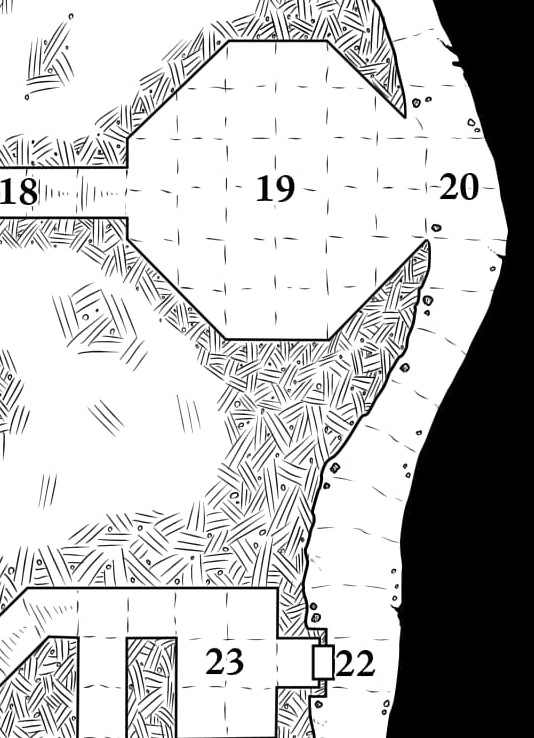
\includegraphics[width=\columnwidth]{pics/map_18-23.jpg}

\subsection{18 : Escaliers}\label{n2:s18}
\begin{itemize}
  \item Couloir de 15m de long, 3m de large et 3m de haut
  \item Air froid, \textbf{silence} total.
  \item Des \textbf{escaliers} s'enfoncent dans les ténèbres.
  \item Une légère brise se fait sentir.
\end{itemize}

La troisième volée de marches est piégée.

\begin{highlight}[Piège]
Dès qu'un poids est appliqué sur la marche
\begin{itemize}
    \item Les marches basculent pour former une rampe de roche lisse
    \item Des épieux jaillissent du sol en bas de l'escalier (1D8 dégâts, 1D4 si sauvegarde Mort)
    \item Se réarme après 5 rounds
\end{itemize}
\end{highlight}

\vfill

\subsection{19 : Arène du Gardien Cobra}\label{n2:s19}
\begin{itemize}
    \item Même forme et taille que \nameref{n2:s11}
    \item Pièce \textbf{octogonale}, avec une \textbf{grande ouverture} à l'est
    \item 18m sur 18m, 5m de haut
    \item \textbf{Arène} froide,
    \item Murs couverts de boucliers divers (des tribus vaincues par les hommes-serpents)
    \begin{itemize}
      \item 5 sont fonctionnels, les autres pourris
      \item 20 PO récupérables en les désassemblant (décorations en argent)
    \end{itemize}
    \item Au centre une statue de pierre en forme de cobra
    \begin{itemize}
      \item \textbf{\nameref{monster:s19}} attaque à vue
    \end{itemize}
\end{itemize}

\subsection{20 : Gouffre et Chemin}\label{n2:s20}
\begin{itemize}
  \item \'Etroit chemin (3m) 24 m jusqu'à \textbf{\nameref{n3:s22}}
  \item \textbf{Glissant} : course ou saut : chute dans le gouffre.
  (sauvegarde contre la mort +5 annule)
  \item \textbf{Gouffre} abyssal à l'est
  \begin{itemize}
    \item large de 18m
    \item mur opposé non visible
  \end{itemize}
\end{itemize}
Si le groupe se met les gobelins fongiques à dos, ils tendent toujours une embuscade ici.
Les gobelins sont collants et ignorent le sol glissant

\subsection{21 : Patelles des Donjons}\label{n2:s21}
\begin{wrapfigure}{l}{0.3\linewidth}
  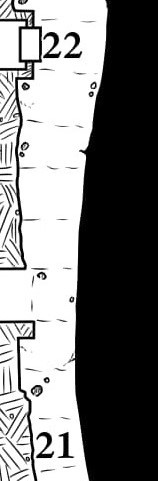
\includegraphics[width=\linewidth]{pics/map_21-22.jpg}
\end{wrapfigure}
Chemin couvert de \textbf{patelles des donjons}:
\begin{itemize}
  \item mollusques à coquille de pierre
  \item \textbf{Contact :} paralysie 1D4 heures (sauvegarde paralysie annule)
  \item \textbf{Paralysé :} dévoré en 1D4 heures
  \item Connu si expérience de donjon
\end{itemize}







